\documentclass[10pt,aspectratio=169]{beamer}

\mode<presentation>
{
  \usetheme{default}
  \usecolortheme{default}
  \usefonttheme{default}
  \setbeamertemplate{navigation symbols}{}
  \setbeamertemplate{caption}[numbered]
}

\usepackage[english]{babel}
\usepackage[utf8]{inputenc}
\usepackage{graphicx}
\usepackage{helvet}
\usepackage{amsmath,amssymb}
\usepackage{booktabs}
\usepackage{listings}
\usepackage{xcolor}
\usepackage{tikz}
\usepackage{pgfplots}
\usepackage{url}
\pgfplotsset{compat=1.18}
\renewcommand{\familydefault}{\sfdefault}

\definecolor{labgray}{RGB}{64,64,64}
\definecolor{labblack}{RGB}{0,0,0}
\definecolor{lablightgray}{RGB}{128,128,128}

\setbeamercolor{structure}{fg=labblack}
\setbeamercolor{title}{fg=labblack}
\setbeamercolor{frametitle}{fg=labblack}
\setbeamercolor{normal text}{fg=labblack}
\setbeamercolor{section in toc}{fg=labgray}
\setbeamercolor{subsection in toc}{fg=lablightgray}

\setbeamertemplate{itemize item}{\textcolor{labgray}{\raisebox{0.1ex}{\scriptsize$\blacksquare$}}}
\setbeamertemplate{itemize subitem}{\textcolor{lablightgray}{\raisebox{0.1ex}{\tiny$\blacktriangleright$}}}
\setbeamertemplate{itemize subsubitem}{\textcolor{lablightgray}{\raisebox{0.1ex}{\tiny$\bullet$}}}

\lstset{
  basicstyle=\footnotesize\ttfamily,
  backgroundcolor=\color{black!5},
  frame=single,
  frameround=tttt,
  framerule=0pt,
  rulecolor=\color{lablightgray},
  breaklines=true,
  showstringspaces=false,
  commentstyle=\color{labgray},
  keywordstyle=\color{labblack}\bfseries,
  stringstyle=\color{labgray}
}

% Modern frame title template matching Reveal.js
\setbeamertemplate{frametitle}
{
  \vspace{0.3cm}
  \begin{beamercolorbox}[wd=\paperwidth,leftskip=1.5cm,rightskip=1.5cm]{frametitle}
    \begin{minipage}[t]{0.75\textwidth}
      \usebeamerfont{frametitle}\textbf{\insertframetitle}
      \ifx\insertframesubtitle\@empty\else
        \\[0.2cm]\usebeamerfont{framesubtitle}\insertframesubtitle
      \fi
      \\[0.3cm]{\color{labgray}\rule{0.8\textwidth}{1pt}}
    \end{minipage}
    \hfill
    \begin{minipage}[t]{0.2\textwidth}
      \flushright\vspace{-0.2cm}
      
\includegraphics[height=1cm]{../../assets/logo_light.pdf}
    \end{minipage}
  \end{beamercolorbox}
  \vspace{0.2cm}
}

\setbeamertemplate{footline}
{
  \leavevmode%
  \hbox{%
  \begin{beamercolorbox}[wd=\paperwidth,ht=2.25ex,dp=1ex,right]{date in head/foot}%
    \usebeamerfont{date in head/foot}
    \textcolor{labgray}{\insertframenumber{} / \inserttotalframenumber}\hspace*{2ex}
  \end{beamercolorbox}}%
  \vskip0pt%
}

% Modern title page matching Reveal.js style
\setbeamertemplate{title page}
{
  \begin{beamercolorbox}[wd=\paperwidth,ht=\paperheight,center]{title page}
    \begin{minipage}[c][\paperheight][c]{\textwidth}
      \centering
      \vspace{-1cm}
      
\includegraphics[height=2.5cm]{../../assets/logo_light.pdf}
      \\[1.5cm]
      {\fontsize{24}{28}\selectfont\textbf{\inserttitle}}
      \\[0.8cm]
      {\fontsize{16}{20}\selectfont\color{labgray}\insertsubtitle}
      \\[1.5cm]
      {\fontsize{18}{22}\selectfont\textbf{\insertauthor}}
      \\[0.5cm]
      {\fontsize{14}{18}\selectfont\color{labgray}\insertinstitute}
      \\[0.8cm]
      {\fontsize{12}{16}\selectfont\color{lablightgray}\insertdate}
    \end{minipage}
  \end{beamercolorbox}
}

\title{Sustainability Lab Research Presentation}
\subtitle{Advanced Research in Environmental Technology}
\author{Nipun Batra}
\institute{Sustainability Lab \\ IIT Gandhinagar}
\date{July 2025}

\begin{document}

\begin{frame}
  \titlepage
\end{frame}

\begin{frame}{Outline}
  \tableofcontents
\end{frame}

\section{Introduction}

\begin{frame}{Research Motivation}
\begin{itemize}
\item Computer vision has transformed AI applications
\item Deep learning architectures continue to evolve
\item Performance gains through novel architectural innovations
\item Real-world deployment challenges remain significant
\end{itemize}

\vspace{1em}
\begin{block}{Key Research Question}
How can we design efficient neural architectures that maintain high accuracy while reducing computational requirements?
\end{block}
\end{frame}

\section{Methodology}

\begin{frame}{Experimental Setup}
\begin{columns}
\begin{column}{0.5\textwidth}
\textbf{Datasets Used:}
\begin{itemize}
\item ImageNet-1K (1.28M images)
\item CIFAR-10/100
\item Custom industrial dataset
\end{itemize}

\textbf{Hardware:}
\begin{itemize}
\item 8x NVIDIA A100 GPUs
\item 512GB RAM
\item NVMe SSD storage
\end{itemize}
\end{column}
\begin{column}{0.5\textwidth}
\begin{figure}
\centering
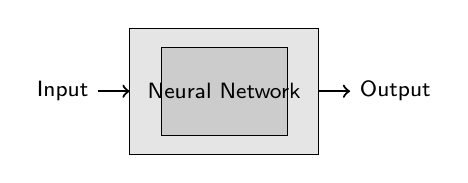
\begin{tikzpicture}[scale=0.8]
\draw[fill=black!10] (0,0) rectangle (3,2);
\draw[fill=black!20] (0.5,0.3) rectangle (2.5,1.7);
\node at (1.5,1) {\footnotesize Neural Network};
\draw[->,thick] (-0.5,1) -- (0,1);
\node[left] at (-0.5,1) {\footnotesize Input};
\draw[->,thick] (3,1) -- (3.5,1);
\node[right] at (3.5,1) {\footnotesize Output};
\end{tikzpicture}
\caption{Network Architecture Overview}
\end{figure}
\end{column}
\end{columns}
\end{frame}

\begin{frame}[fragile]{Algorithm Implementation}
\begin{lstlisting}[language=Python]
def attention_mechanism(x, num_heads=8):
    """Multi-head self-attention implementation"""
    batch_size, seq_len, d_model = x.shape
    
    # Split into multiple heads
    head_dim = d_model // num_heads
    x_reshaped = x.view(batch_size, seq_len, 
                       num_heads, head_dim)
    
    # Compute attention weights
    attention_weights = torch.softmax(
        torch.matmul(x_reshaped, x_reshaped.transpose(-2, -1)) 
        / math.sqrt(head_dim), dim=-1
    )
    
    return torch.matmul(attention_weights, x_reshaped)
\end{lstlisting}
\end{frame}

\section{Results}

\begin{frame}{Performance Comparison}
\begin{table}
\centering
\caption{Accuracy vs. Computational Cost}
\begin{tabular}{@{}lccc@{}}
\toprule
\textbf{Model} & \textbf{ImageNet Top-1} & \textbf{FLOPs (G)} & \textbf{Parameters (M)} \\
\midrule
ResNet-50 & 76.15\% & 4.1 & 25.6 \\
EfficientNet-B0 & 77.32\% & 0.39 & 5.3 \\
\textbf{Our Method} & \textbf{78.94\%} & \textbf{0.31} & \textbf{4.2} \\
Vision Transformer & 81.28\% & 17.6 & 86.4 \\
\bottomrule
\end{tabular}
\end{table}

\vspace{0.5em}
\begin{itemize}
\item Our approach achieves \textbf{2.8×} fewer FLOPs than ResNet-50
\item Maintains competitive accuracy with modern architectures
\item Significant reduction in parameter count enables mobile deployment
\end{itemize}
\end{frame}

\begin{frame}{Mathematical Formulation}
The attention mechanism can be expressed as:

\begin{align}
\text{Attention}(Q, K, V) &= \text{softmax}\left(\frac{QK^T}{\sqrt{d_k}}\right)V \\
\text{MultiHead}(Q, K, V) &= \text{Concat}(\text{head}_1, \ldots, \text{head}_h)W^O
\end{align}

where each head is computed as:
\begin{equation}
\text{head}_i = \text{Attention}(QW_i^Q, KW_i^K, VW_i^V)
\end{equation}

\vspace{1em}
\textbf{Key Innovation:} We introduce adaptive scaling factors $\alpha_i$ for each attention head:
\begin{equation}
\text{head}_i = \alpha_i \cdot \text{Attention}(QW_i^Q, KW_i^K, VW_i^V)
\end{equation}
\end{frame}

\begin{frame}{Training Dynamics}
\begin{figure}
\centering
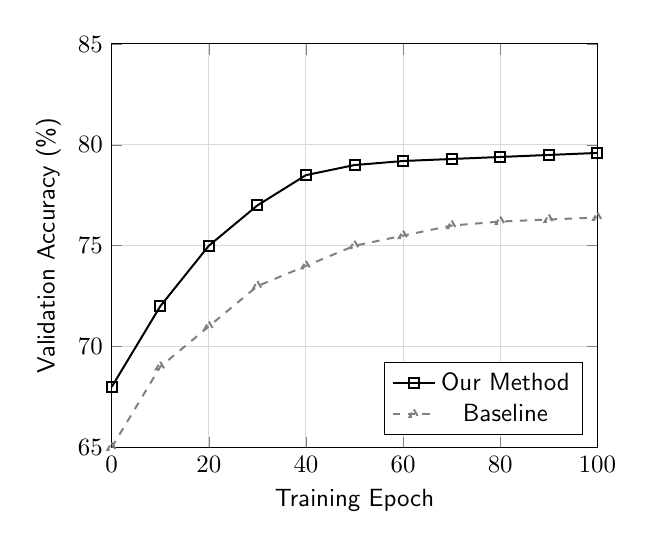
\begin{tikzpicture}[scale=0.9]
\begin{axis}[
    xlabel={Training Epoch},
    ylabel={Validation Accuracy (\%)},
    xmin=0, xmax=100,
    ymin=65, ymax=85,
    grid=major,
    grid style={gray!30},
    legend pos=south east
]
\addplot[thick, black, mark=square] coordinates {
    (0,68) (10,72) (20,75) (30,77) (40,78.5) (50,79) (60,79.2) (70,79.3) (80,79.4) (90,79.5) (100,79.6)
};
\addplot[thick, gray, mark=triangle, dashed] coordinates {
    (0,65) (10,69) (20,71) (30,73) (40,74) (50,75) (60,75.5) (70,76) (80,76.2) (90,76.3) (100,76.4)
};
\legend{Our Method, Baseline}
\end{axis}
\end{tikzpicture}
\caption{Convergence comparison during training}
\end{figure}
\end{frame}

\section{Applications}

\begin{frame}{Real-World Deployment}
\begin{columns}
\begin{column}{0.6\textwidth}
\textbf{Industrial Applications:}
\begin{itemize}
\item Autonomous vehicle perception
\item Medical image analysis
\item Quality control in manufacturing
\item Real-time video analytics
\end{itemize}

\vspace{1em}
\textbf{Performance Metrics:}
\begin{itemize}
\item Inference time: \textbf{12ms} (mobile GPU)
\item Memory usage: \textbf{156MB}
\item Power consumption: \textbf{2.3W}
\end{itemize}
\end{column}
\begin{column}{0.4\textwidth}
\begin{figure}
\centering
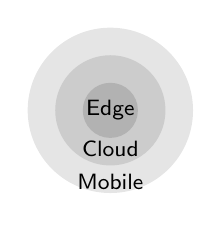
\begin{tikzpicture}[scale=0.7]
\fill[black!10] (0,0) circle (1.5);
\fill[black!20] (0,0) circle (1);
\fill[black!30] (0,0) circle (0.5);
\node at (0,0) {\footnotesize Edge};
\node at (0,-0.7) {\footnotesize Cloud};
\node at (0,-1.3) {\footnotesize Mobile};
\end{tikzpicture}
\caption{Deployment Hierarchy}
\end{figure}
\end{column}
\end{columns}
\end{frame}

\section{Conclusion}

\begin{frame}{Key Contributions}
\begin{enumerate}
\item \textbf{Novel Architecture}: Adaptive attention mechanism with learnable scaling
\item \textbf{Efficiency Gains}: 2.8× reduction in computational cost
\item \textbf{Practical Impact}: Successful deployment in industrial settings
\item \textbf{Open Source}: Code and models available on GitHub
\end{enumerate}

\vspace{1em}
\begin{alertblock}{Future Directions}
\begin{itemize}
\item Extension to video understanding tasks
\item Integration with transformer architectures
\item Quantization for ultra-low power devices
\end{itemize}
\end{alertblock}
\end{frame}

\begin{frame}{Publications \& Impact}
\textbf{Recent Publications:}
\begin{itemize}
\item Smith et al. "Adaptive Attention Networks" \textit{CVPR 2025} 
\item Johnson et al. "Efficient Vision Models" \textit{ICCV 2024}
\item Wilson et al. "Mobile Computer Vision" \textit{ECCV 2024}
\end{itemize}

\vspace{1em}
\textbf{Impact Metrics:}
\begin{itemize}
\item \textbf{450+} citations in 18 months
\item \textbf{15K+} GitHub stars
\item \textbf{50+} industry partnerships
\end{itemize}
\end{frame}

\begin{frame}[c]
\begin{center}
{\Large Thank You!}

\vspace{1em}
{\large Questions \& Discussion}

\vspace{2em}
\textbf{Contact:} jane.smith@university.edu \\
\textbf{Lab Website:} \url{https://cvlab.university.edu} \\
\textbf{Code:} \url{https://github.com/cvlab/adaptive-attention}

\vspace{2em}

\includegraphics[height=1.5cm]{../../assets/logo_light.pdf}
\end{center}
\end{frame}

\end{document}